\documentclass{article}

\usepackage{amsmath,amsfonts,tikz}

\newcommand{\ii}{\mathbf{i}}
\newcommand{\jj}{\mathbf{j}}
\newcommand{\kk}{\mathbf{k}}
\newcommand{\rr}{\mathbf{r}}
\newcommand{\vv}{\mathbf{v}}
\newcommand{\aaa}{\mathbf{a}}
\newcommand{\TT}{\mathbf{T}}
\newcommand{\NN}{\mathbf{N}}
\newcommand{\BB}{\mathbf{B}}

\begin{document}

{\bf Worksheet \#25; date: 04/19/2018}

{\bf MATH 53 Multivariable Calculus}

\begin{enumerate}
\item {\em True / False?} Fix two points $A$ and $B$ in a simply connected domain $D$. If $\int_C \mathbf{F} \cdot d\rr$ is the same for all paths $C$ from $A$ to $B$, then $\mathbf{F}$ must be conservative on $D$.

\item {\em True / False?} Suppose $P$ and $Q$ has continuous partial derivatives everywhere. Green's Theorem cannot help us in computing line integral $\int_C \mathbf{F} \cdot d\rr$ where $C$ is given below.
\begin{center}
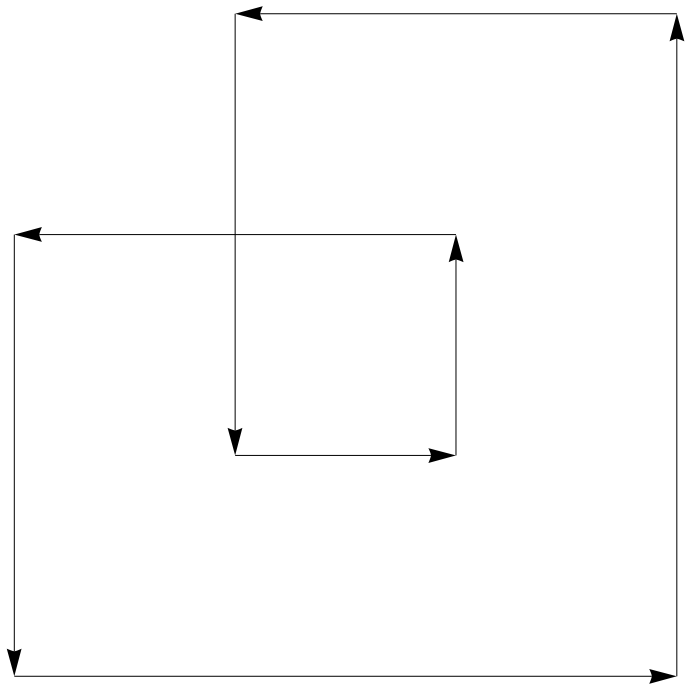
\includegraphics[width=0.33\textwidth]{quiz12dis114pic}
\end{center}

\item {\em True / False?} Fix two points $A$ and $B$ in a domain $D$. If $\int_C \mathbf{F} \cdot d\rr$ is the same for all paths $C$ from $A$ to $B$, then $\mathbf{F}$ must be conservative on $D$.

\item {\em True / False?} Here is another proof of Green's Theorem with holes in it: Suppose the region with hole is $D'$, the hole itself is $D_2$ and the region $D'$ with the hole filled is $D_1$. The outer and inner boundaries are $C_1$ and $C_2$. We can then apply Green's Theorem to $D_1$ and $D_2$, and subtract one integral from the other.

\item {\em (Concept check)} What are the symbols for grad, div, curl respectively? What sort of objects does the operator $\nabla$, $\nabla \cdot$, $\nabla \times$ and $\nabla^2$ take as input? What sort of objects are the output? Write $\nabla^2$ in terms of the other operators.

\item {\em (Stewart 16.5.7)} Compute the curl and the divergence of the vector field
\[
\mathbf{F}(x, y, z) = \langle e^x \sin y, e^y \sin z, e^z \sin x\rangle
\]

\item {\em (Stewart 16.5.17)} Determine whether or not the vector field is conservative. If it is conservative, find a function $f$ such that $\mathbf{F} = \nabla f$.
\[
\mathbf{F}(x, y, z) = e^{yz} \ii + xz e^{yz} \jj + xy e^{yz} \kk
\]

\item {\em (Stewart 16.5.19)} Is there a vector field $\mathbf{G}$ on $\mathbf{R}^3$ such that $\text{curl} \mathbf{G} = \langle x \sin y, \cos y, z - xy \rangle$? Explain.

\item {\em (Concept check)} What is ``conservative'', ``irrotational'' and ``incompressible''?

\item {\em (Stewart 16.5.27)} Prove the identity
\[
\text{div}(\mathbf{F} \times \mathbf{G}) = \mathbf{G} \cdot \text{curl } \mathbf{F} - \mathbf{F} \cdot \text{curl } \mathbf{G}
\]

\item {\em (Stewart 16.5.29)} Prove the identity
\[
\text{curl}(\text{curl }\mathbf{F}) = \text{grad}(\text{div }\mathbf{F}) - \nabla^2 \mathbf{F}
\]
\end{enumerate}

\end{document}